\begin{center}
\begin{minipage}{\textwidth} 
    \hspace{2.0cm}
    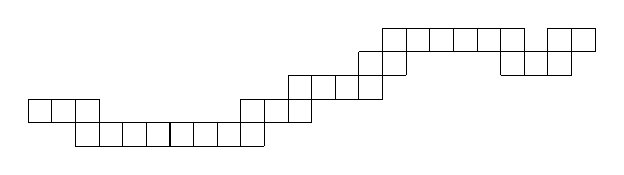
\begin{tikzpicture}[scale=0.3pt]
        \def\a{-5.5}
        \def\b{10.5}

        \draw[color = black!100] (0, 2) -- (3, 2);
        \draw[color = black!100] (0, 3) -- (3, 3);

        \foreach \x in {0, ..., 3} {
            \draw[color = black!100] (\x, 2) -- (\x, 2+1);
        }

        \draw[color = black!100] (2, 1) -- (10, 1);
        \draw[color = black!100] (2, 2) -- (10, 2);

        \foreach \x in {2, ..., 10} {
            \draw[color = black!100] (\x, 1) -- (\x, 1+1);
        }

        \draw[color = black!100] (9, 2) -- (12, 2);
        \draw[color = black!100] (9, 3) -- (12, 3);

        \foreach \x in {9, ..., 12} {
            \draw[color = black!100] (\x, 2) -- (\x, 2+1);
        }

        \draw[color = black!100] (11, 3) -- (15, 3);
        \draw[color = black!100] (11, 4) -- (15, 4);

         \foreach \x in {11, ..., 15} {
            \draw[color = black!100] (\x, 3) -- (\x, 3+1);
        }

        \draw[color = black!100] (14, 4) -- (16, 4);
        \draw[color = black!100] (14, 5) -- (16, 5);

         \foreach \x in {14, ..., 16} {
            \draw[color = black!100] (\x, 4) -- (\x, 4+1);
        }

        \draw[color = black!100] (15, 5) -- (21, 5);
        \draw[color = black!100] (15, 6) -- (21, 6); 
        \foreach \x in {15, ..., 21} {
            \draw[color = black!100] (\x, 5) -- (\x, 5+1);
        }

        \draw[color = black!100] (20, 4) -- (23, 4);
        \draw[color = black!100] (20, 5) -- (23, 5); 
        \foreach \x in {20, ..., 23} {
            \draw[color = black!100] (\x, 4) -- (\x, 4+1);
        }

        \draw[color = black!100] (22, 5) -- (24, 5);
        \draw[color = black!100] (22, 6) -- (24, 6);
        \foreach \x in {22, ..., 24} {
            \draw[color = black!100] (\x, 5) -- (\x, 5+1);
        }
    \end{tikzpicture}
\end{minipage}
\vspace{1.1cm}

\begin{minipage}{\textwidth}
    \hspace{2.0cm}
    \begin{tikzpicture}[scale=0.3pt]
        \def\a{-5.5}
        \def\b{10.5}

        \draw[color = black!100] (0, 2) -- (3, 2);
        \draw[color = black!100] (0, 3) -- (3, 3);

        \foreach \x in {0, ..., 3} {
            \draw[color = black!100] (\x, 2) -- (\x, 2+1);
        }

        \draw[color = black!100] (0, 3) -- (3, 3);
        \draw[color = black!100] (0, 4) -- (3, 4);

        \foreach \x in {0, ..., 3} {
            \draw[color = black!100] (\x, 3) -- (\x, 3+1);
        }

        \draw[color = black!100] (2, 1) -- (13, 1);
        \draw[color = black!100] (2, 2) -- (13, 2);

        \foreach \x in {2, ..., 13} {
            \draw[color = black!100] (\x, 1) -- (\x, 1+1);
        }

        \draw[color = black!100] (10, 2) -- (11, 2);
        \draw[color = black!100] (10, 3) -- (11, 3);

        \foreach \x in {10, 11} {
            \draw[color = black!100] (\x, 2) -- (\x, 2+1);
        }

        \draw[color = black!100] (9, 3) -- (15, 3);
        \draw[color = black!100] (9, 4) -- (15, 4);

         \foreach \x in {9, ..., 15} {
            \draw[color = black!100] (\x, 3) -- (\x, 3+1);
        }

        \draw[color = black!100] (14, 4) -- (17, 4);
        \draw[color = black!100] (14, 5) -- (17, 5);

         \foreach \x in {14, ..., 17} {
            \draw[color = black!100] (\x, 4) -- (\x, 4+1);
        }

        \draw[color = black!100] (8, 4) -- (11, 4);
        \draw[color = black!100] (8, 5) -- (11, 5);

         \foreach \x in {8, ..., 11} {
            \draw[color = black!100] (\x, 4) -- (\x, 4+1);
        }

        \draw (7.5,2.5) pic[red] {cross=30pt};
    \end{tikzpicture}
\end{minipage}
\end{center}